
\documentclass{article}
\usepackage{enumerate}
\usepackage{algorithm}
\usepackage{algorithmic} % pesudo code
\usepackage{tikz}
\usetikzlibrary{positioning,shapes,arrows}

\usepackage{amsmath,amsfonts,amsthm} % Math packages
\usepackage{graphicx}
\usepackage{caption}
\usepackage{subcaption}

\newcommand{\norm}[1]{\left\lVert #1 \right\rVert}
\newtheoremstyle{quest}{\topsep}{\topsep}{}{}{\bfseries}{}{ }{\thmname{#1}\thmnote{ #3}.}
\theoremstyle{quest}
\newtheorem*{question}{Question}

\begin{document}
\section*{Nearest Neighbor, Decision Trees, Neural Networks}
\begin{question}[1]
\end{question}
\begin{enumerate}[a.]
\item 
Decision Trees. Because the target function is in disjunctive normal form, that's exatly what rules Decision Tree algorithm can generate. Besides we have enough data.
\item
Nearest Neighbour. Because the expected value of $\sum x_i$ for both classes is fixed, the dimension of this problem can be reduced to 1, and it's linear separable. Nearest Neighbour(distance measured by $\sum x_i$) is better due to the small size of the dataset.
\item
None. $\norm{\mathbf{x}}$ is 100, so there are $2^{100}$ instance of $\mathbf{x}$ with different permutation of 0 and 1. Thus instance-based approach Nearest Neighbour is hit by curse of dimensinality. The same with Decision Trees, because to approach the function in disjunctive normal form the complexity is the same. How about the magical Neural Networks? Maybe it will work with 100 layers, but we should consider data we have and overfitting. This function is hard to learn, because each feature is independent, and you can gain none information by individual feature untill you check all the features. 
\item
Neural Networks. The function looks complex, but all the formula can be represent by Neural Networks, because the feature is binary, $x_i*x_j$ equal to $x_i\  and\  x_j$, $x_i / (x_j+\epsilon)$ can also be represent with $x_0$ and hidden layer.

\begin{figure}
	\centering
	\begin{subfigure}[hb]{0.7\textwidth}
		\includegraphics[width=\textwidth]{test1.eps}
		\caption{Error of Neural Network on $b$.}
		\label{fig:10-0}
	\end{subfigure}
	\hfill
	\begin{subfigure}[hb]{0.7\textwidth}
		\includegraphics[width=\textwidth]{test2.eps}
		\caption{Confusion Matrix of Neural Network on $b$.}
		\label{fig:10-2}
	\end{subfigure}
	\caption{Some result of my tiny experiment.}\label{f11}
\end{figure}
For $b$ and $d$, I also make experiments(using Matlab) comparing the performance of Nearest Neighbour and Neural Networks, because I think both classifiers can work with the given function and data. For $b$, the original Nearest Neighbour(without using $\sum x_i$ as distance measurement, because obiviously the NN described in $b$ can work, I don't  think it needs to be test) achieve 50\% percision, while Neural Networks(with 10 neurons and one hidden layer) achieve 93\% percision(as figure~\ref{f11} shows). For $d$, my experiment show Nearest Neighbour achieve percision around 70\%, while Neural Networks achieve 100\% percision on both training and test set(both have 10000 instances). I think the reason behind this result is that I do not add $\epsilon$(noise) in the data. I randomly generate the data, then assign instance with target value by exatly the target function. In this case, the result means Neural Networks can perfectly represent the target function, while nearest neighbour do have an effect, but due to it's an instance-based approach, it can not represent the target function very well.

\end{enumerate}
\begin{question}[2]
\end{question}
The dataset shown in figure~\ref{q2}:\\
\begin{center}
\begin{tabular}{c|c|c} \hline
$x_1$ & $x_2$ & y \\ \hline
1 & 1 & 1 \\ 
1 & 2 & 1 \\ 
2 & 2 & 1 \\ 
-1.25 & -1.75 & 1 \\ 
-1 & -1 & 0 \\ 
-1 & -2 & 0 \\ 
-2 & -2 & 0 \\ 
1.25 & 1.75 & 0 \\ \hline
\end{tabular}
\end{center}


\begin{figure}[h!]
\centering
\includegraphics[scale=0.5]{q2.eps}
\caption{The dataset for Question 2} \label{q2}
\end{figure}

\section*{Perceptrons}
\begin{question}[3]
\end{question}
See figure~\ref{f2}.
\begin{figure}[h!]
\centering
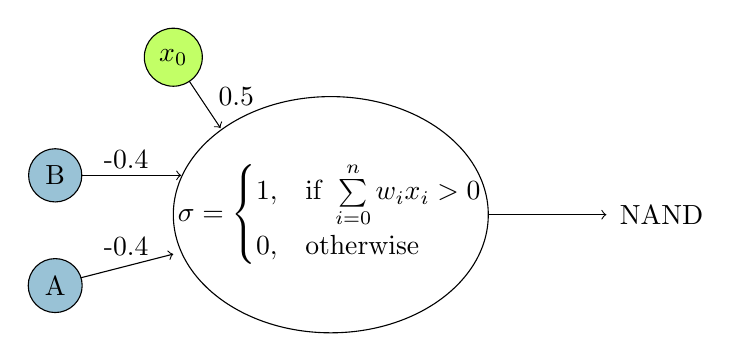
\begin{tikzpicture}
\draw  (0,2.6) node[fill=blue!60!green!40, circle, draw]{A};
\draw (0,4) node[fill=blue!60!green!40, circle, draw]{B};
\draw (1.5, 5.5) node[fill=green!40!yellow!60, circle, draw]{$x_0$};
\draw (3.5, 3.5) ellipse (2cm and 1.5cm);
\draw (3.5, 3.5) node{$\sigma = \begin{cases}
1, & \text{if } \sum\limits_{i=0}^n w_ix_i > 0 \\
0, & \text{otherwise}
\end{cases}$};
\draw [->] (0.33, 2.7) -- (1.5, 3);
\draw [->] (0.33, 4) -- (1.6, 4);
\draw [->] (1.7, 5.2 ) -- (2.1, 4.6);
\draw [->] (5.5, 3.5) -- (7, 3.5);
\draw (7.7, 3.5) node{NAND};
\draw (2.3, 5) node{0.5};
\draw (0.9, 3.1) node{-0.4};
\draw (0.9, 4.2) node{-0.4};
\end{tikzpicture}
\caption{NAND Perceptron} \label{f2}
\label{a1}
\end{figure}
\section*{Optimization}
\begin{question}[4]
\end{question}
Mutation and crossover.
\begin{question}[5]
\end{question}
\begin{enumerate}[a.]
\item
The optimization problem is:
$${\underset  {x}{\operatorname {arg\,min}}}\,f(x)$$
where $f(x)$ is a sawtooth wave function as figure~\ref{f3} shows (in discrete form, we can think this is a digital signal).\\
\begin{figure}[h!]
\centering
\includegraphics[scale=0.2]{f3.eps}
\caption{Sawtooth wave.} \label{f3}
\end{figure}
The sawtooth(triangle also) wave has properties that every local minima or maxima is also global minima or maxima and it's non differentiable in some points. Gradient Descent can not handle non differentiable function, and to find a local minima Hill Climbing has a better efficiency and more reliable than Gentic Algorithms. 

So Hill Climbing is a better choice for this problem.
\item
Find the minimal of the graph (generated by data interpolation), and we know it approximates to $f(\mathbf{x,y,z}) =\mathbf{x}^2+\mathbf{y}^2+\mathbf{z}^2$) as figure~\ref{f4} shows. \\
\begin{figure}[h!]
\centering
\includegraphics[scale=0.9]{f4.eps}
\caption{} \label{f4}
\end{figure}

For this problem, Gradient Descent is better, since the function is continous and convex. And it may converge faster than Hill Climbing, because this is a 3-dimension problem, in each iteration hill climbing will try to make change in one dimension, while gradient descent will go forward on the direction with steepest gradient.
\item
Also an unconstrained optimization problem: find the minimal of $f(x)$. But here $f(x)$ is non-convex and has saddle point(s), so both Hill Climbing and Gradient Descent will not work well. We can suppose this problem occur when we want to use manifold learning for feature selection. Thus encoding the feature vector is not difficult for Genetic Algorithms. 

So for this problem, Genetic Algorithms is better.
\end{enumerate}
\section*{Bayes Nets and Statistical Estimation}
\begin{question}[6]
\end{question}
\begin{enumerate}[a.]
\item
See figure~\ref{f5}.
\begin{figure}[h!]
\centering
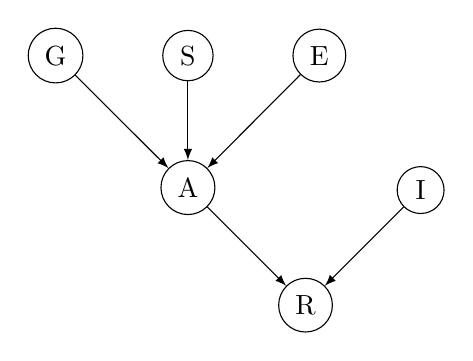
\begin{tikzpicture}
\node[draw, circle] (ng) {G};
\node[draw, circle, right=of ng] (ns) {S};
\node[draw, circle, right=of ns] (ne) {E};
\node[draw, circle, below=of ns] (na) {A};
\node[draw, circle, below right=of na] (nr) {R};
\node[draw, circle, above right=of nr] (ni) {I};
\path (ng) edge[-latex] (na)
(ns) edge[-latex] (na) 
(ne) edge[-latex] (na)
(na) edge[-latex] (nr)
(ni) edge[-latex] (nr);
\end{tikzpicture}
\caption{Bayes Net.} \label{f5}
\end{figure}
\item
$1+1+1+2^3+2^2=3+8+4=15$
\item
$2^6-1=63$
\item
Yes, because $E$ is not a descendant of $G$ and vice versa, and both $G$ and $E$ do not have parent in the graph, so they are uncorrelated.
\item
Yes, because if we know $A$, $E$ and $G$ is d-separated by $A$, so $E$ and $G$ are conditional independent given $A$.
\end{enumerate}
\begin{question}[7]
\end{question}
\begin{enumerate}[a.]
\item
\begin{align*} 
P(C) & =\sum\limits_{i}\sum\limits_{j}P(C| A_i, B_j)P(A_i, B_j) \\ 
& = \sum\limits_{i}\sum\limits_{j}P(C| A_i, B_j)P(A_i)P(B_j)\\
& = 0.35+0.35+0.7*0.3*0.5+0.3*0.3*0.5 \\
& = 0.85
\end{align*}
\item
$9/12=0.75$
\end{enumerate}
\end{document}